\subsubsection{Description de {\em Verif-correl}}
La d\'ecision de  {\em Verif-correl} intervient dans le choix de la partition coh\'erente.
En effet, la partition coh\'erente utilise la loi de conservation des noeuds \cite{loiDeConservation} sur les mesures physiques. Cette loi \'enonce que la diff\'erence entre la somme des flots entrants et sortants d'un noeud du r\'eseau est inf\'erieure \'a la valeur $\epsilon$ des pertes par effets joules.
\newline
Soit une clique $C$ partitionn\'e en deux sous-ensembles $C_{u1}$ et $C_{u2}$. 
Le sous-ensemble $C_{u1}$ d\'esigne l'ensemble des arcs entrants dans le sommet $C$ du r\'eseau electrique et ce sommet correspond \`a une clique dans le line-graphe.
Le sous-ensemble $C_{u2}$ d\'esigne aussi l'ensemble des arcs sortants dans le sommet $C$.
Le flot du sommet $a_i \in C_{u1}$ est le vecteur de mesures $gp_{a_i}^{x}$ avec  $x \in GP^{a_i}$ la grandeur physique et $gp_{a_i}^{x}[t]$ une mesure physique. 
De m\^eme, le vecteur de mesures $gp_{a_j}^{x}$  avec $a_j \in C_{u2}$ un sommet et $gp_{a_j}^{x}[t]$ une mesure physique est le flot du sommet $a_j$ de l'ensemble $C_{u2}$. 
Nous rappelons que la grandeur $x$ a un vecteur de mesures pour toutes les sommets de $C$.
$$ \forall a_i , a_j \in C, x \in GP^{a_i} \cap GP^{a_j} $$
La fonction {\em Verif-correl} retourne une valeur bool\'eenne. Elle retourne {\em Vrai} ou $1$ si la diff\'erence de la somme des mesures entrantes et sortantes d'un sommet \`a chaque instant $t$ est inf\'erieure \`a $\epsilon$
$$ Verif-correl(C_{u1}, C_{u2}) = 1 \Leftrightarrow  \sum_{i = 1}^{|C1|} gp_{a_i}^{x}(t) - \sum_{j = 1}^{|C2|} gp_{a_j}^{x}(t)  \le \epsilon $$
Ainsi $ Verif-correl(C_{u1}, C_{u2}) = 1$ signifie que l'ambigu\''{i}t\'e autour du sommet $C$ est lev\'ee et la partition de $(C_{u1}, C_{u2})$ est correcte.
\newline
Nous consid\'erons que la fonction {\em Verif-correl} retourne toujours $1$. Cela implique que la valeur $\epsilon$ dans le r\'eseau est donn\'ee. Dans le cas o\`u cette valeur $\epsilon$ est inconnue, quel est la valeur minimum de ces pertes  \`a partir de laquelle la partition est toujours exacte?



\subsubsection{Impact des pertes par effets joules}
%epsilon est le taux min des pertes par effets joules pour lequel l'oracle ne comet pas d'erreurs.
% EJ ce sont les pertes par effet joules dans le reseau.
Nous consid\'erons que le r\'eseau \'electrique modelis\'e par un DAG $G$ est connu et que sa matrice de corr\'elation est correcte. 
Dans le but d'\'etudier le taux minimum des pertes par effets joules not\'ee $\epsilon$ dans le r\'eseau afin que la partition coh\'erente propos\'ee par  {\em Verif-correl} soit toujours correcte, 
nous cherchons les ensembles arcs entrants $S_1$ et sortants $S_2$ d'un sommet tel que $Verif-correl(S_1, S_2) = 1$.
Nous d\'efinissons la similarit\'e comme \'etant le pourcentage d'arcs bien pr\'edits par rapport aux arcs de $G$. 
Nous r\'ealisons deux exp\'eriences: 
\begin{itemize}
\item La premi\`ere exp\'erience consiste \`a g\'en\'erer des mesures de flots de divers graphes en faisant varier, de $0$ \`a $1$ par pas de $0.125$, les pertes par effets joules $EJ$ tout en fixant la variable $\epsilon$. Nous ex\'ecutons l'algorithme de couverture sur diff\'erents graphes, chaque graphe ayant un $EJ \in [0,1]$. Nous \'etudions l'\'evolution de la  similarit\'e en fonction de pertes joules $EJ$. 

\item La deuxi\`eme exp\'erience consiste \`a faire varier la variable $\epsilon$ en fixant la similarit\'e \`a $1$.  Nous \'etudions les variations des pertes en fonctions de $\epsilon$.  Les pertes par effets joules $EJ$ varient  de $0$ \`a $1$ par pas de $0.125$. 

\end{itemize}
Rappelons que $EJ=0.1$ signifie qu'il existe une diff\'erence de flot par grandeurs de $0.1$ entre les arcs ext\'erieures (sortantes) et int\'erieures (entrantes) \`a chaque sommet. Ainsi $EJ=0$ signifiant qu'il n'existe aucune perte tandis que  $EJ=1$ signifiant qu'il n'existe aucuns flots entre les arcs entrants et sortants d'un sommet du r\'eseau de flots.
% experience 1
\paragraph{exp\'erience 1} :
On fixe  $\epsilon=0.75$. 
La figure \ref{courbeEJCoef} resume les variations de {\em Verif-correl}. 
Le fait que la courbe de la variable $\epsilon$ est d\'ecroissante confirme notre hypoth\`ese selon laquelle il n'existe aucuns flots entre les arcs entrants et sortants d'un sommet lorsque les pertes par effets joules sont \'egales \`a $EJ = 1$. En effet, pour toute valeur de pertes par effets joules  $EJ=[0,0.3]$, le graphe propos\'e est identique au graphe du r\'eseau \'electrique. Par contre, {\em Verif-correl} se trompe deux sur trois sur les cliques fournies pour $EJ = ]0.3,0.9]$ parce que la coefficent de similarit\'e est de $0.38$. 

%experience 2
\paragraph{exp\'erience 2} :
Ici, on suppose la similarit\'e \'egale \`a $1$ et on cherche les variations de la variable $\epsilon$ en fonction des pertes par {\em effets joules}. 
Les pertes par {\em effets joules} varient de $[0,1]$ par pas de $0.125$ et nous distinguons $8$ intervalles [0,0.125], ]0.125,0.250], ]0.250,0.375], ]0.375,0.5], ]0.5,0.625], ]0.625, 0.75], ]0.75,0.875], ]0.875,1]. 
Pour chaque valeur $\epsilon$, on compte les intervalles $EJ_x, x \in [1,8]$ dans lesquelles la similarit\'e est \'egale \`a $1$ not\'e $X(\epsilon)$. Ainsi $X(\epsilon=0.3) = 8$ signifie que  les pertes par effets joules varient de $0$ \`a $1$ (EJ=[0,1]) et $X(\epsilon=0.3) = 2$ correspond \`a une variation de $EJ$ sur l'intervalle $[0,0.250]$.
On cr\'ee ainsi la distribution de $\epsilon$ en fonction des pertes par effets joules.
La figure \ref{courbeEpsilonEJ}  r\'esume cette distribution qui varie de $1$ (correspondant \`a une variation sur [0,0.125]) \`a $8$ (correspondant \`a une variation sur [0,1]).
La courbe de cette distribution est constante de l'intervalle $\epsilon = [0,0.125]$ puis  d\'ecroissante de l'intervalle $\epsilon =[0.125,1]$ et cette pente est tr\`es accentu\'ee dans l'intervalle $\epsilon = [0.8, 1]$. 
Au d\'el\`a  de $\epsilon > 0.8$, les pertes par effets joules varient dans l'intervalle $EJ=[0,0.2]$.
On en conclut que le meilleur intervalle est $\epsilon = [0.8, 1]$ pour produire des graphes de similarit\'e \'egale \`a $1$ en pr\'esence de pertes par {\em effets joules} de $20\%$.

% images
\begin{figure}
\centering
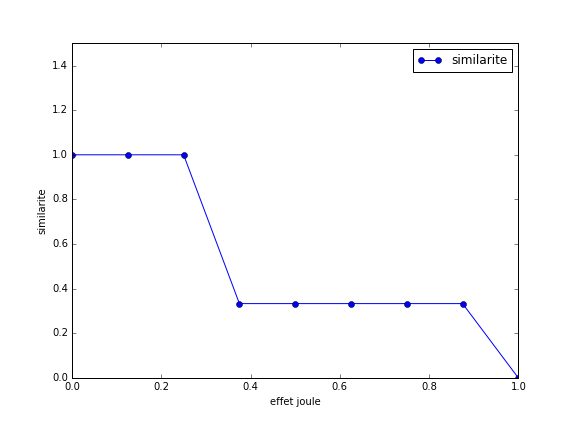
\includegraphics[scale=0.50]{courbe_similarite_selon_EJ_pour_epsilon_075.png}
\caption{ Le coefficient de similarit\'e en fonction des pertes par {\em effets joules} pour $epsilon=0.75$.}
\label {courbeEJCoef}
\end{figure}
\begin{figure}
\centering
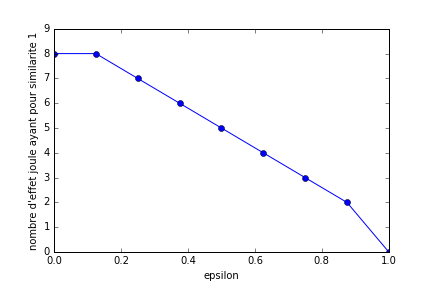
\includegraphics[scale=0.65]{courbe_epsilon_selon_nbreEJ_pour_similarite_1.png}
\caption{ Relation inverse entre $\epsilon$ et $EJ$: $8$ en ordonn\'e correspond \`a $[0,1]$, $7$ \`a $[0, 0.875]$ }
\label {courbeEpsilonEJ}
\end{figure}

% conclusion
Ces deux exp\'eriences montrent que la d\'ecision de la fonction {\em Verif-correl}  a une r\'elation inverse avec les pertes par effets joules ($EJ$). En effet, plus $\epsilon$ est petit plus les pertes par effets joules sont grandes et plus les d\'ecisions de {\em Verif-correl} sont erron\'ees.
\begin{equation}
	\epsilon > 1 - EJ
\end{equation}
